% How the Nerfacto backbone was replaced by ZipNeRF inside FruitNeRF
% Build:  pdflatex backbone_swap.tex   (run twice)
\documentclass[aspectratio=169,11pt]{beamer}

\usetheme{default}
\usecolortheme{default}
\usepackage[T1]{fontenc}
\usepackage[utf8]{inputenc}
\usepackage{booktabs}
\usepackage{xcolor}
\usepackage{tikz}
\usetikzlibrary{arrows.meta,positioning,fit,backgrounds,calc,shapes.geometric}

\definecolor{ink}{HTML}{0B0B0B}
\definecolor{ink2}{HTML}{52514E}
\definecolor{zipblue}{HTML}{2A78D6}
\definecolor{fnorange}{HTML}{EB6834}
\definecolor{surface}{HTML}{FCFCFB}
\definecolor{keepgreen}{HTML}{2F7D51}
\definecolor{rule}{HTML}{C9C7C2}

\setbeamercolor{normal text}{fg=ink,bg=surface}
\setbeamercolor{frametitle}{fg=ink,bg=surface}
\setbeamercolor{structure}{fg=zipblue}
\setbeamerfont{frametitle}{size=\large,series=\bfseries}
\setbeamertemplate{navigation symbols}{}
\setbeamertemplate{footline}[frame number]
\setbeamertemplate{itemize items}[circle]
\beamertemplatenavigationsymbolsempty

\newcommand{\zn}{\textcolor{zipblue}{\texttt{fruit\_zipnerf}}}
\newcommand{\fn}{\textcolor{fnorange}{\texttt{fruit\_nerf}}}

% ---- shared node styles -------------------------------------------------
\tikzset{
  blk/.style   = {rounded corners=2pt, draw=rule, line width=0.7pt,
                  fill=white, align=center, inner sep=5pt, font=\footnotesize},
  keep/.style  = {blk, draw=keepgreen, fill=keepgreen!7, text=ink},
  old/.style   = {blk, draw=fnorange, fill=fnorange!8, text=ink},
  new/.style   = {blk, draw=zipblue, fill=zipblue!8, text=ink},
  ghost/.style = {blk, draw=rule, fill=black!3, text=ink2},
  fl/.style    = {-{Stealth[length=4pt]}, draw=ink2, line width=0.7pt},
  lbl/.style   = {font=\scriptsize\itshape, text=ink2},
}

\title{Swapping the backbone: Nerfacto $\rightarrow$ ZipNeRF}
\subtitle{What \texttt{fruit\_zipnerf} changes inside FruitNeRF, and what it leaves alone}
\author{Nicol\'as Araya}
\date{\today}

\begin{document}

\begin{frame}[plain]
  \titlepage
\end{frame}

% ==================================================================
\begin{frame}{The whole change, in one picture}

  \begin{center}
  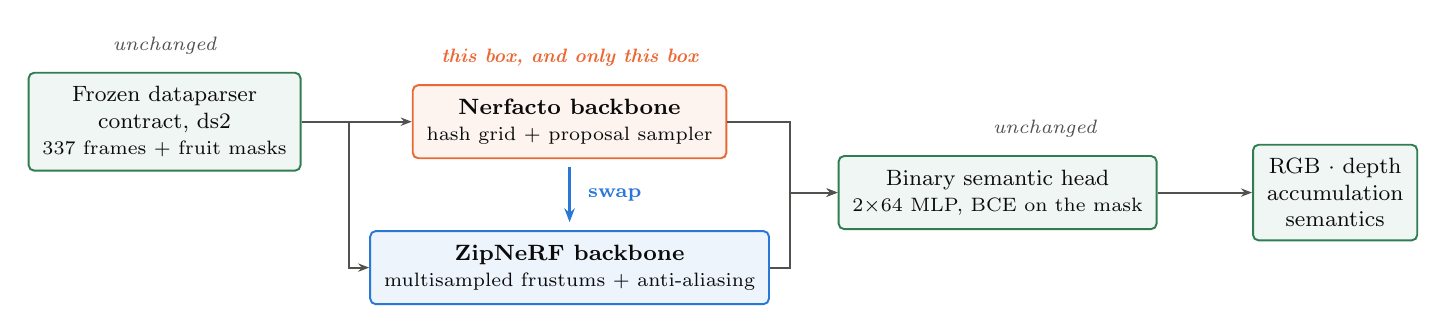
\begin{tikzpicture}[node distance=8mm]

    % --- unchanged front of the pipeline
    \node[keep] (data) {Frozen dataparser\\contract, ds2\\{\scriptsize 337 frames + fruit masks}};

    % --- the swapped middle
    \node[old,  right=14mm of data, minimum width=30mm] (nerfacto)
      {\textbf{Nerfacto backbone}\\{\scriptsize hash grid $+$ proposal sampler}};
    \node[new,  below=9mm of nerfacto, minimum width=30mm] (zip)
      {\textbf{ZipNeRF backbone}\\{\scriptsize multisampled frustums $+$ anti-aliasing}};

    % --- unchanged back of the pipeline
    \node[keep, right=14mm of nerfacto, yshift=-9mm] (head)
      {Binary semantic head\\{\scriptsize 2$\times$64 MLP, BCE on the mask}};
    \node[keep, right=12mm of head] (out)
      {RGB $\cdot$ depth\\accumulation\\semantics};

    % --- flow
    \draw[fl] (data.east) -- ++(6mm,0) |- (nerfacto.west);
    \draw[fl] (data.east) -- ++(6mm,0) |- (zip.west);
    \draw[fl] (nerfacto.east) -| ($(head.west)+(-6mm,0)$) -- (head.west);
    \draw[fl] (zip.east)      -| ($(head.west)+(-6mm,0)$) -- (head.west);
    \draw[fl] (head) -- (out);

    % --- the swap arrow
    \draw[-{Stealth[length=5pt]}, zipblue, line width=1.1pt]
      ($(nerfacto.south)+(0,-1mm)$) -- ($(zip.north)+(0,1mm)$)
      node[midway, right=1mm, font=\scriptsize\bfseries, text=zipblue] {swap};

    % --- banners
    \node[lbl, above=1mm of data]     {unchanged};
    \node[lbl, above=1mm of nerfacto] {\textcolor{fnorange}{\textbf{this box, and only this box}}};
    \node[lbl, above=1mm of head, xshift=6mm] {unchanged};

  \end{tikzpicture}
  \end{center}

  \vspace{0.2em}
  {\small The semantic head, its BCE loss, the masks and the dataparser contract are
   byte-for-byte the same. \fn{} and \zn{} differ in the geometry backbone.}
\end{frame}

% ==================================================================
\begin{frame}{What the backbone actually does differently}

  \begin{center}
  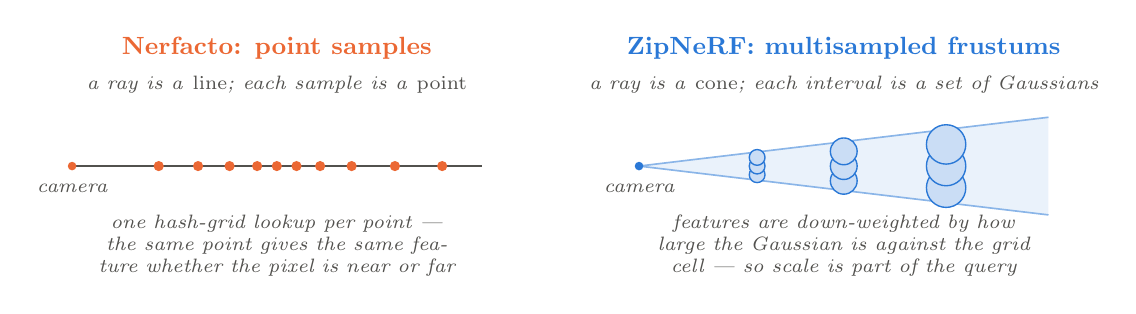
\begin{tikzpicture}

    % ---------------- Nerfacto : point samples on a ray
    \begin{scope}[shift={(0,0)}]
      \node[font=\small\bfseries, text=fnorange] at (2.6,1.5) {Nerfacto: point samples};
      \draw[draw=ink2, line width=0.7pt] (0,0) -- (5.2,0);
      \node[circle, fill=fnorange, inner sep=1.1pt] at (0,0) {};
      \node[lbl, below=1mm] at (0,0) {camera};
      \foreach \x in {1.1,1.6,2.0,2.35,2.6,2.85,3.15,3.55,4.1,4.7}{
        \node[circle, fill=fnorange, inner sep=1.3pt] at (\x,0) {};
      }
      \node[lbl, above=8mm, align=center] at (2.6,0)
        {a ray is a \emph{line}; each sample is a \emph{point}};
      \node[lbl, below=5mm, align=center, text width=52mm] at (2.6,0)
        {one hash-grid lookup per point --- the same point gives the same
         feature whether the pixel is near or far};
    \end{scope}

    % ---------------- ZipNeRF : multisampled conical frustum
    \begin{scope}[shift={(7.2,0)}]
      \node[font=\small\bfseries, text=zipblue] at (2.6,1.5) {ZipNeRF: multisampled frustums};
      \fill[zipblue!10] (0,0) -- (5.2,0.62) -- (5.2,-0.62) -- cycle;
      \draw[draw=zipblue!55, line width=0.6pt] (0,0) -- (5.2,0.62);
      \draw[draw=zipblue!55, line width=0.6pt] (0,0) -- (5.2,-0.62);
      \node[circle, fill=zipblue, inner sep=1.1pt] at (0,0) {};
      \node[lbl, below=1mm] at (0,0) {camera};
      % a few intervals, each drawn as a set of little gaussians
      \foreach \x/\r in {1.5/0.10, 2.6/0.17, 3.9/0.25}{
        \foreach \dy in {-1,0,1}{
          \draw[draw=zipblue, fill=zipblue!25, line width=0.5pt]
            (\x, \dy*\r*1.1) circle (\r);
        }
      }
      \node[lbl, above=8mm, align=center] at (2.6,0)
        {a ray is a \emph{cone}; each interval is a set of Gaussians};
      \node[lbl, below=5mm, align=center, text width=54mm] at (2.6,0)
        {features are down-weighted by how large the Gaussian is against the
         grid cell --- so scale is part of the query};
    \end{scope}

  \end{tikzpicture}
  \end{center}

  \vspace{0.6em}
  {\small That is the anti-aliasing: a cherry seen from 2\,m and from 20\,cm no
   longer lands on the same grid features.}
\end{frame}

% ==================================================================
\begin{frame}{Inside the swapped box}

  \begin{center}
  \resizebox{\textwidth}{!}{%
  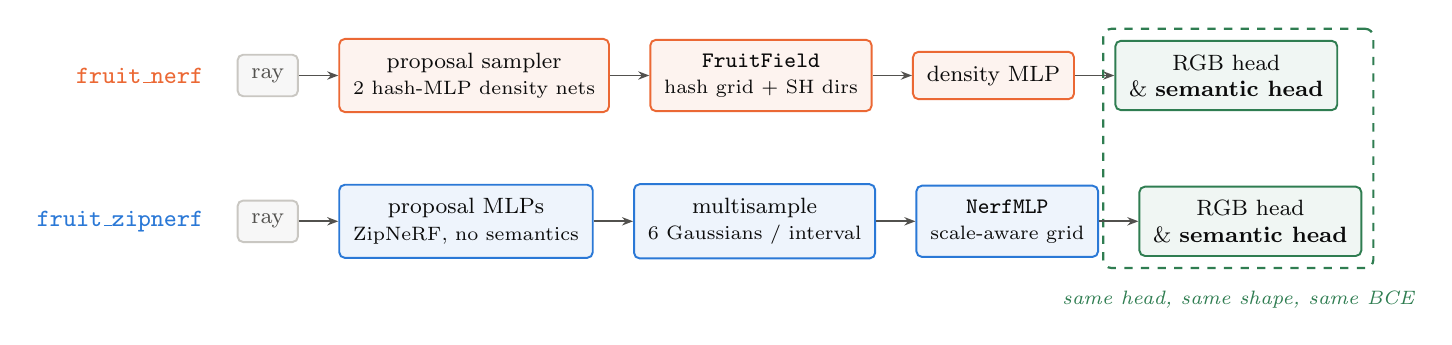
\begin{tikzpicture}[node distance=6mm]

    % ---- top row: fruit_nerf
    \node[ghost] (a1) {ray};
    \node[old, right=5mm of a1]  (a2) {proposal sampler\\{\scriptsize 2 hash-MLP density nets}};
    \node[old, right=5mm of a2]  (a3) {\texttt{FruitField}\\{\scriptsize hash grid $+$ SH dirs}};
    \node[old, right=5mm of a3]  (a4) {density MLP};
    \node[keep, right=5mm of a4] (a5) {RGB head\\ \& \textbf{semantic head}};
    \node[left=3mm of a1, font=\small\bfseries, text=fnorange] {\fn};

    % ---- bottom row: fruit_zipnerf
    \node[ghost, below=13mm of a1] (b1) {ray};
    \node[new, right=5mm of b1]  (b2) {proposal MLPs\\{\scriptsize ZipNeRF, no semantics}};
    \node[new, right=5mm of b2]  (b3) {multisample\\{\scriptsize 6 Gaussians / interval}};
    \node[new, right=5mm of b3]  (b4) {\texttt{NerfMLP}\\{\scriptsize scale-aware grid}};
    \node[keep, right=5mm of b4] (b5) {RGB head\\ \& \textbf{semantic head}};
    \node[left=3mm of b1, font=\small\bfseries, text=zipblue] {\zn};

    \foreach \i/\j in {a1/a2, a2/a3, a3/a4, a4/a5, b1/b2, b2/b3, b3/b4, b4/b5}{
      \draw[fl] (\i) -- (\j);
    }

    % ---- the identical head
    \begin{scope}[on background layer]
      \node[draw=keepgreen, dashed, line width=0.8pt, rounded corners=3pt,
            fit=(a5)(b5), inner sep=4pt] (box) {};
    \end{scope}
    \node[lbl, text=keepgreen, below=1.5mm of box]
      {same head, same shape, same BCE};

  \end{tikzpicture}}
  \end{center}

  \vspace{0.4em}
  {\small The semantic head is switched on through gin on the \texttt{NerfMLP}
   only. The proposal MLPs stay untouched: they exist to place samples, and
   FruitNeRF likewise reads semantics only from the main field.}
\end{frame}

% ==================================================================
\begin{frame}{Honest caveat: it is not a backbone-only A/B}

  \begin{center}
  \small
  \begin{tabular}{lll}
    \toprule
      & \fn & \zn \\
    \midrule
    Semantic head        & 2$\times$64 MLP, BCE       & \textbf{identical} \\
    Masks / dataparser   & frozen contract, ds2       & \textbf{identical} \\
    Sampling             & points on a ray            & multisampled frustums \\
    Interlevel loss      & nerfacto interlevel        & \texttt{anti\_interlevel} (camp spline) \\
    \textcolor{fnorange}{Distortion loss}
                         & \textcolor{fnorange}{\textbf{computed but inert}}
                         & \textcolor{zipblue}{\textbf{live gradient}} \\
    \textcolor{fnorange}{LR schedule}
                         & \multicolumn{2}{l}{\textcolor{fnorange}{\textbf{not matched between the two}}} \\
    \bottomrule
  \end{tabular}
  \end{center}

  \vspace{0.9em}
  \begin{itemize}
    \item In \fn{} the distortion loss reaches \texttt{metrics\_dict} only --- the
          \texttt{0.002} in \texttt{config.yml} is a no-op. In \zn{} it is a real
          gradient (\texttt{power\_ladder} on metric \texttt{tdist}).
    \item So the measured \textbf{+1.05\,dB} is ``ZipNeRF recipe'' vs
          ``Nerfacto recipe'', not the backbone in isolation.
    \item Semantic F1 does not move ($0.594 \to 0.592$): the head was never the
          bottleneck.
  \end{itemize}
\end{frame}

\end{document}
